%!TEX root = ../thesis.tex
% ******************************* Thesis Appendix B ********************************

\chapter{Supplementary Figures}

\section{Additional results from Chapter 3}

\begin{figure}[h]
    \centering
    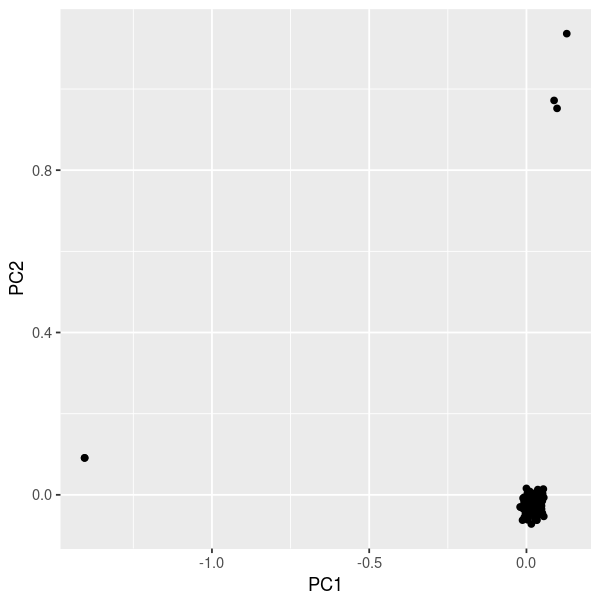
\includegraphics[width=10cm]{Appendix2/Fig/supplement_genotype_pcs.png}
    \caption[Population structure of donors included in the study]{\textbf{Population structure of donors included in the study.} \\
    Principal component (PC) decomposition of the kinship matrix (calculated using plink \cite{purcell2007plink}) across all cell lines included in our study.
    The four outlier cell lines were excluded from the analyses described in \textbf{section \ref{sec:best_practice}}.}
    \label{suppl_fig:kinship_pcs}
\end{figure}

\begin{figure}[h]
    \centering
    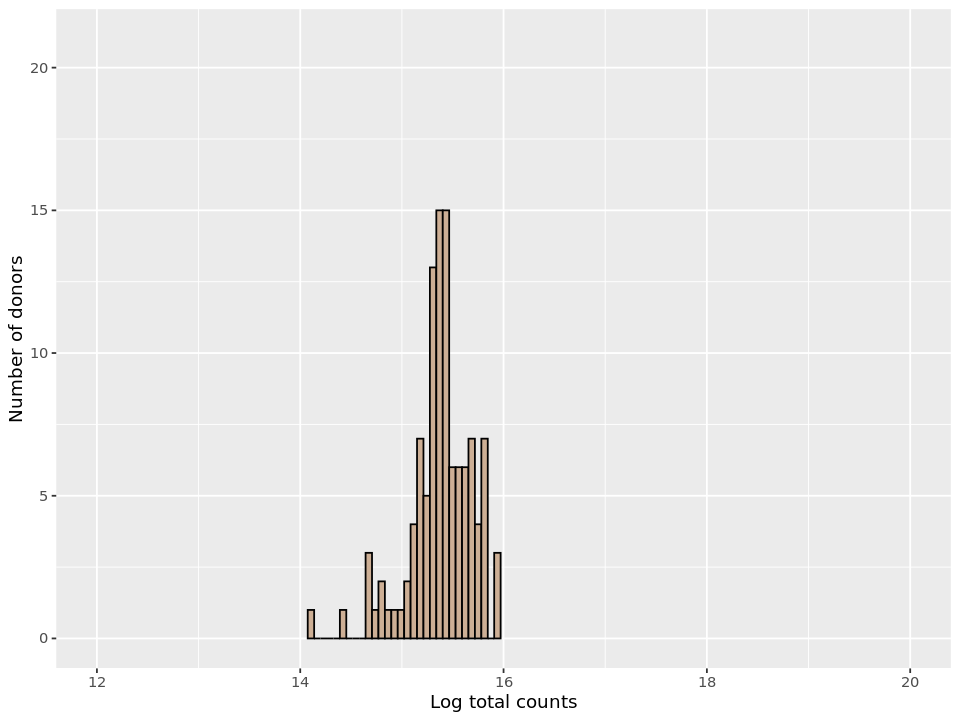
\includegraphics[width=12cm]{Appendix2/Fig/suppl_distribution_fixed_ncells.png}
    \caption[Distribution of total reads scRNA-seq same number of cells per donor]{Distribution of total reads from a scRNA-seq dataset, when considering the same number of cells for each donor.
    Same as \textbf{Fig. \ref{fig:sc_bulk_counts}}, but downsampling to the same number of cells (n=10) from each donor.}
    \label{suppl_fig:counts_sc_ncells}
\end{figure}

\begin{figure}[h]
    \centering
    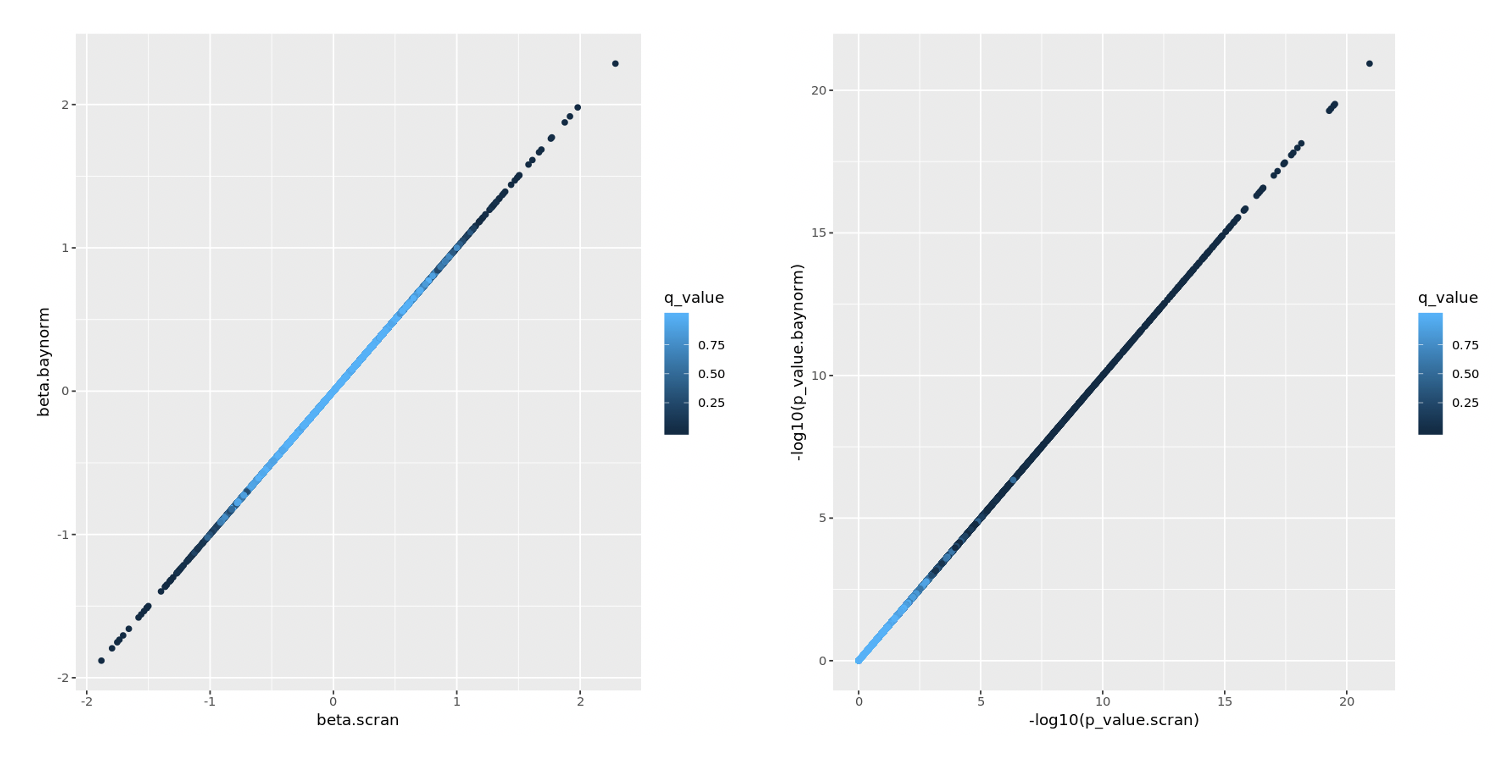
\includegraphics[width=16cm]{Appendix2/Fig/suppl_scran_vs_baynorm.png}
    \caption[Correlation of results between scran and baynorm normalisation]{\textbf{Correlation of results between scran and baynorm normalisation.}\\
    Scatter plots of eQTL effect sizes (left) and p values (right) obtained when testing association of iPSC mean eQTL discovered after normalising counts using scran (x axis) or baynorm (y axis).}
    \label{suppl_fig:scran_vs_baynorm}
\end{figure}

\clearpage

\section{Additional results Chapter 4}

\begin{figure}[h]
    \centering
    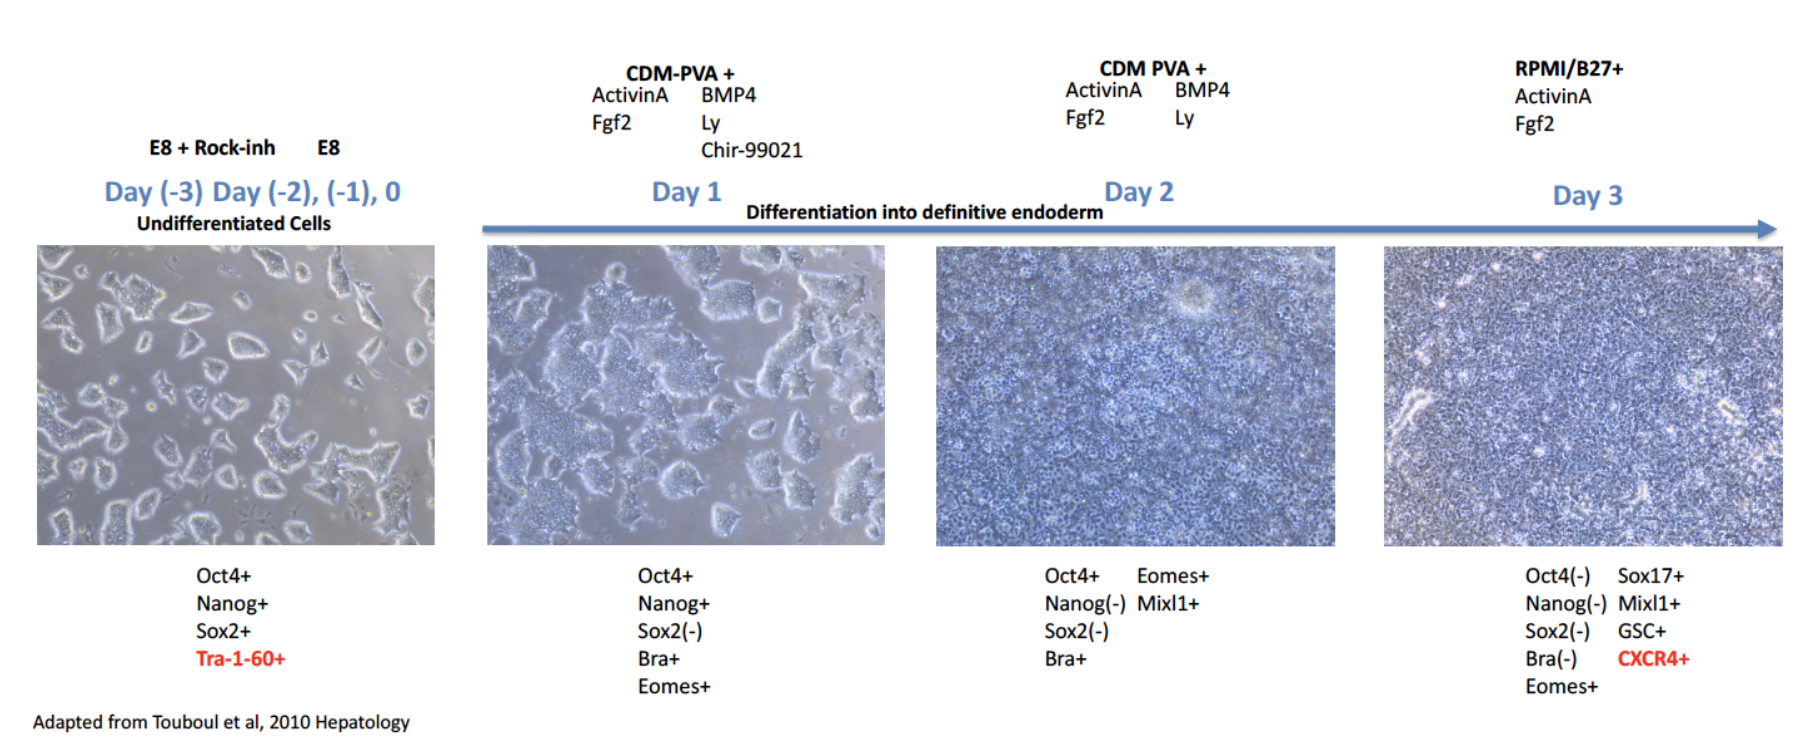
\includegraphics[width=16cm]{Appendix2/Fig/suppl_protocol.png}
    \caption[Endoderm differentiation protocol]{\textbf{Endoderm differentiation protocol.}\\
    Schematic representation of the chemically defined protocol used to initiate differentiation towards  definitive endoderm (adapted from \cite{touboul2010generation}). 
    Tra-1-60 and CXCR4 are canonical cell surface markers used to sort live cells by differentiation stage. }
    \label{suppl_fig:endodiff_exp_protocol}
\end{figure}

\begin{figure}[h]
    \centering
    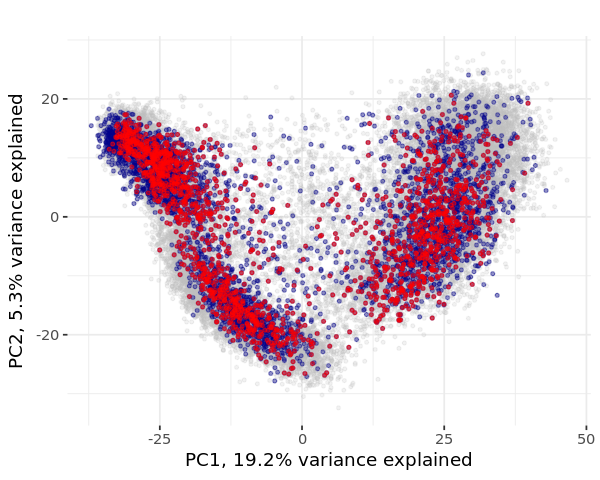
\includegraphics[width=15cm]{Appendix2/Fig/suppl_diabetes_lines.png}
    \caption[PCA of healthy and diseased cell lines]{Comparison of expression patterns between healthy and diseased cell lines.
    PCA and t-SNE representations of cells from neonatal diabetes lines, compared to healthy lines from the same experiments. 
    (A) PCA plot for cells from the neonatal diabetes cell lines (red), cells from healthy lines from the same seven experiments (dark blue), against the background of all cells (grey). 
    (B) t-SNE plot of the same cells as in A.}
    \label{suppl_fig:pca_diabetes_lines}
\end{figure}

% FACS?

\clearpage

\section{Additional results Chapter 5}

\begin{figure}[h]
    \centering
    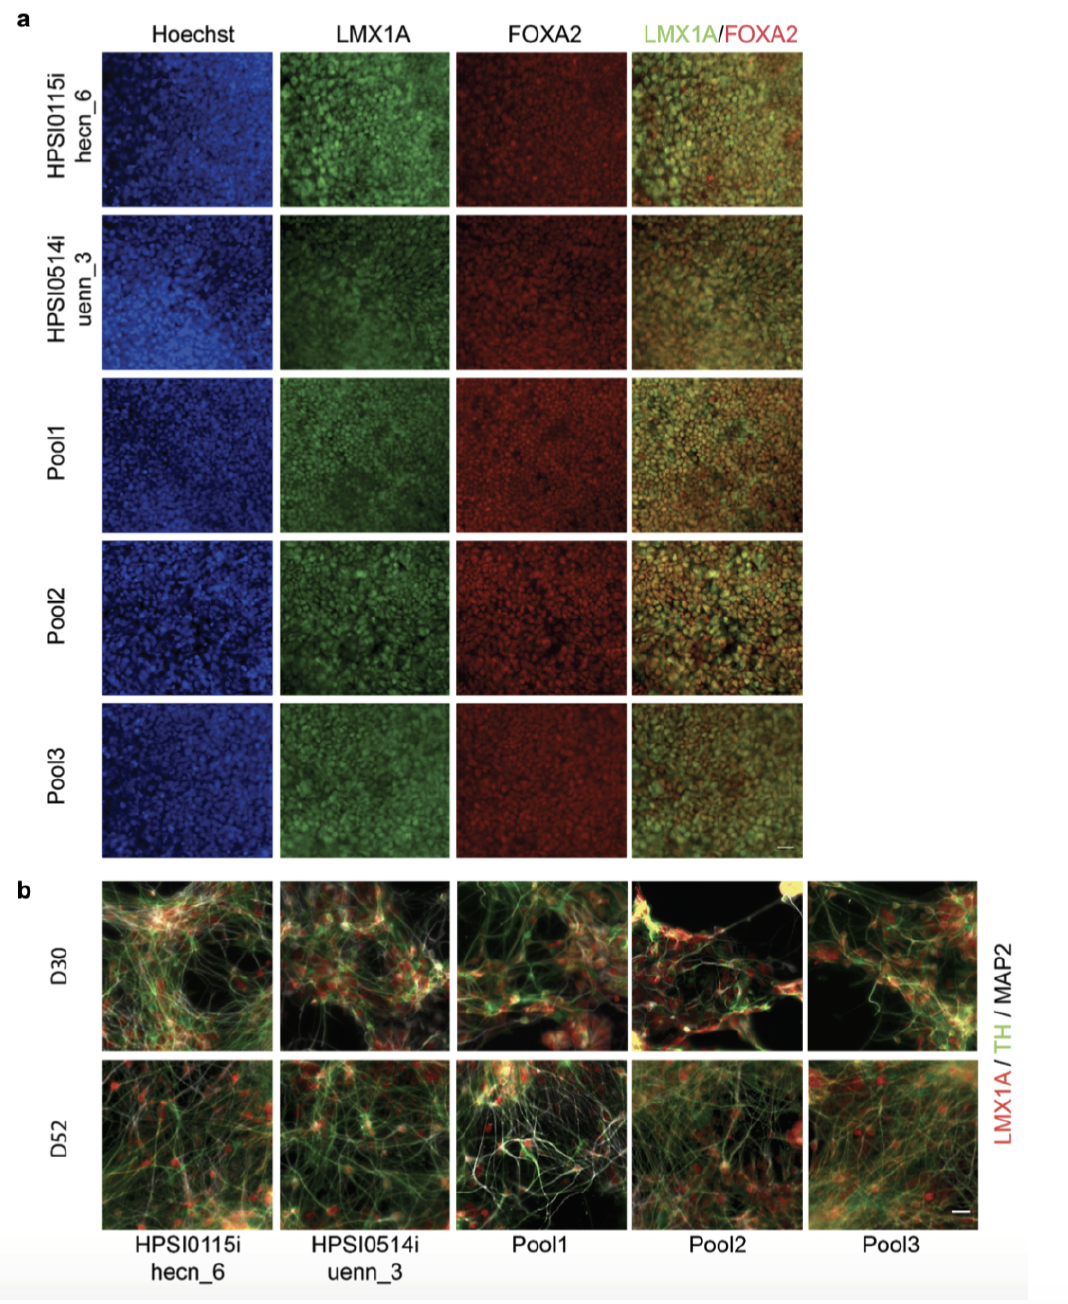
\includegraphics[width=14cm]{Appendix2/Fig/suppl_neuroseq_immunostaining.png}
    \caption[Immunostaining of midbrain neural progenitors and dopaminergic neurons]{\textbf{Immunostaining of midbrain neural progenitors and dopaminergic neurons.}\\
    Figure by Julie Jerber.
    (a) Immunostaining for known midbrain progenitor markers LMX1A and FOXA2 at day 11. 
    Nuclei were counterstained with Hoechst. 
    Scale bar: 25µm. 
    (b) Immunostaining of differentiated dopaminergic neurons for  the neuronal marker MAPT2 (white) and the dopaminergic neuronal markers TH and LMX1A. 
    Scale bar: 25µm. 
    Data is shown for two example individual cell lines (HPSI0155i-hecn\_6 and HPSI0514i-uenn\_3) as well as three entire differentiation pools (Pools 1,2,3).}
    \label{suppl_fig:immunostaining}
\end{figure}


\begin{figure}[h]
    \centering
    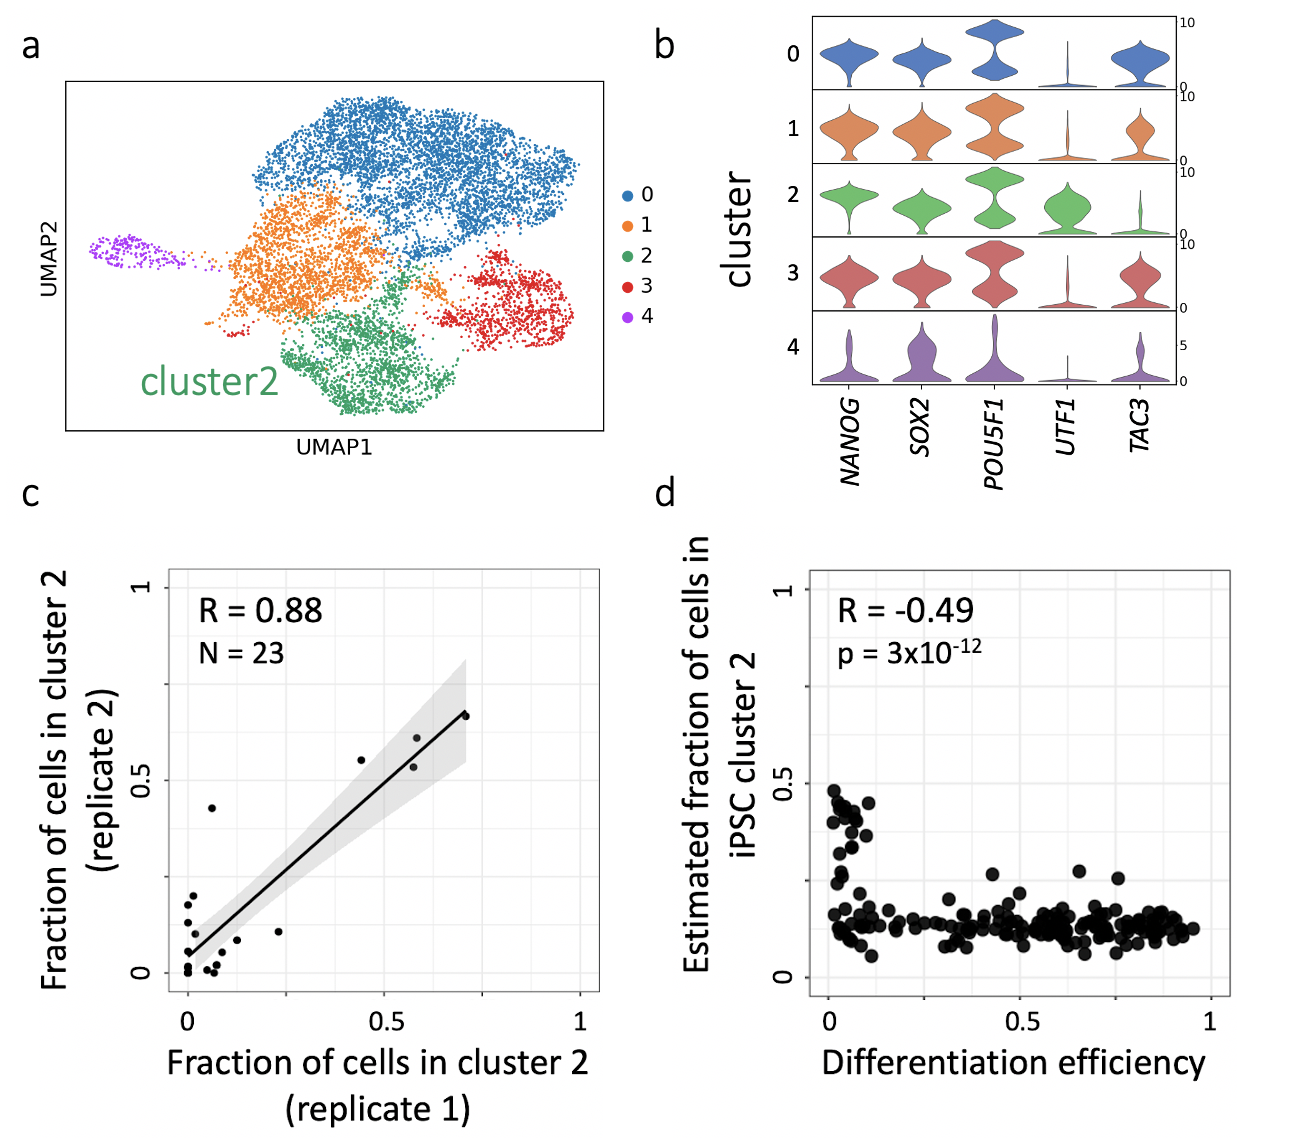
\includegraphics[width=15cm]{Appendix2/Fig/suppl_ips_cluster2.png}
    \caption[An iPSC sub-population is associated with lower differentiation efficiency]{\textbf{Re-analysis of iPSC scRNA-seq data reveals a subpopulation characterised by expression of predictive marker genes associated with lower neural differentiation efficiency.}\\
     (a) UMAP overview of the dataset. 
     iPSC scRNA-seq data from \cite{cuomo2020single} were re-analysed following the same batch correction and clustering steps applied to our neural differentiation data, identifying 5 clusters. 
     (b) Violin plots of gene expression for genes related to pluripotency (\textit{NANOG, SOX2, POU5F1}) and two gene markers that are respectively upregulated and downregulated in cluster 2 (\textit{UTF1, TAC3}, from \textbf{Fig. \ref{fig:neuroseq_ips_expression_signature}}). 
     (c) Scatter plot showing the proportion of cells assigned to cluster 2 between replicates (n=23). 
     (d) Scatterplot between the proportion of cells assigned to cluster 2 (y-axis) and differentiation efficiency (x-axis) similar to \textbf{Fig \ref{fig:neuroseq_ips_sc_genes}c} but where we use imputed proportions of cluster 2 cells from bulk RNA-seq available for most cell lines (n=182).}
    \label{suppl_fig:ipsc_cluster2}
\end{figure}


\begin{figure}[h]
    \centering
    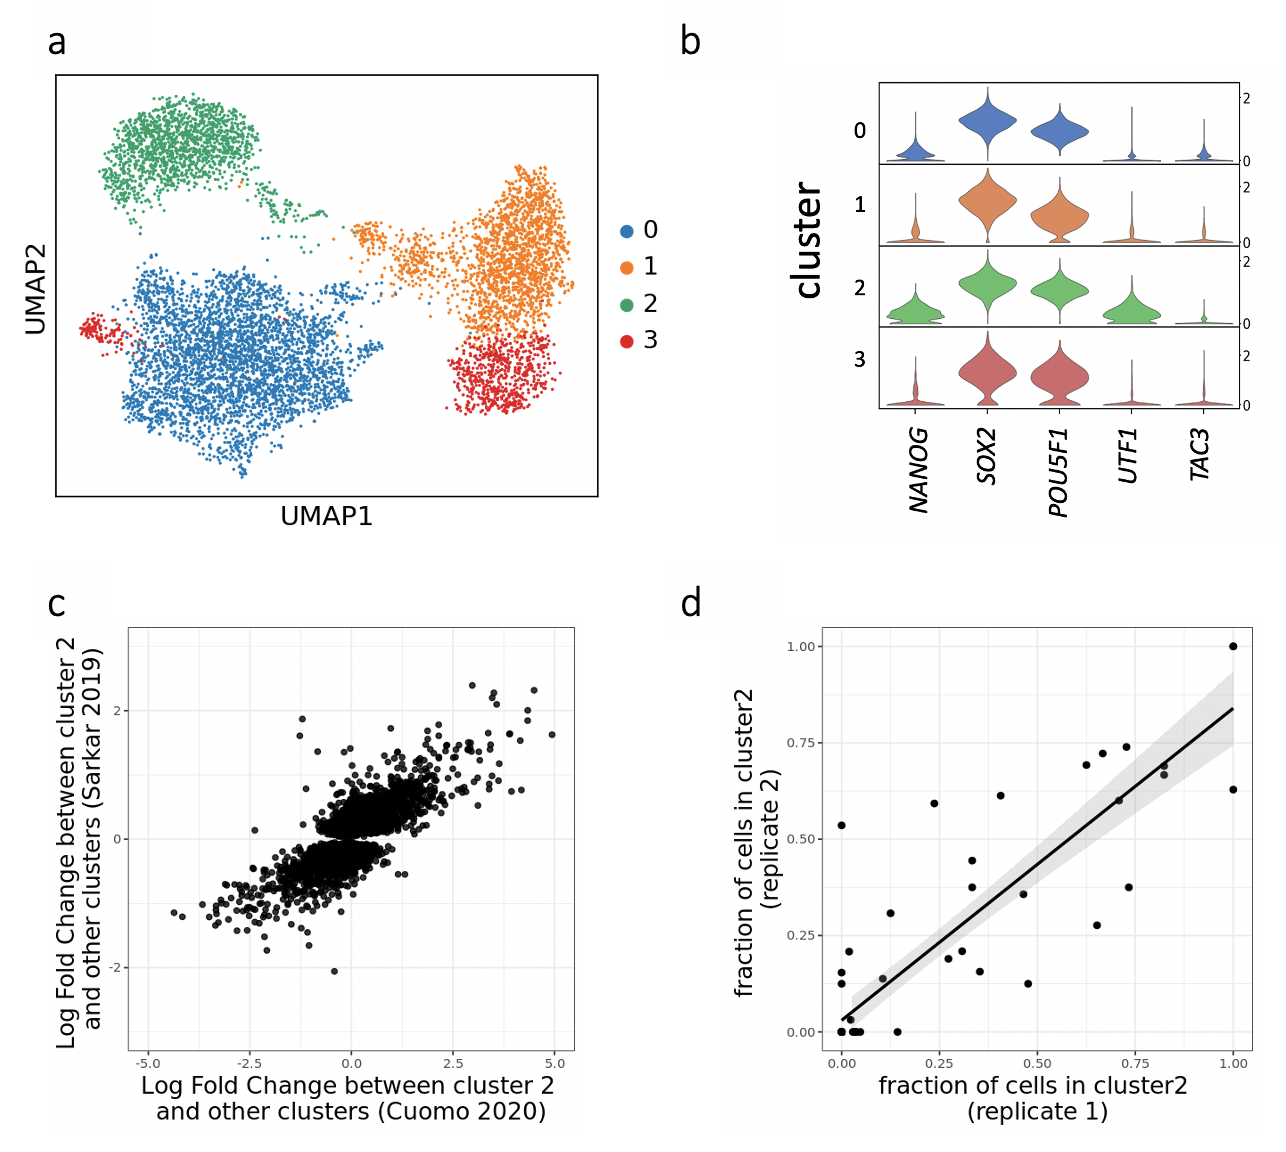
\includegraphics[width=16cm]{Appendix2/Fig/suppl_ipsc_cluster2_sarkar.png}
    \caption[Analysis of a single cell iPSC dataset from Sarkar \textit{et al.}]{\textbf{Analysis of a single cell iPSC dataset from Sarkar \textit{et al.}}\\
    (a) UMAP overview of the dataset. 
    iPSC scRNA-seq data from \cite{sarkar2019discovery} were re-analysed following the same data normalisation and clustering steps applied to our neural differentiation data, identifying 4 clusters. 
    (b) Violin plots of gene expression for genes related to pluripotency (\textit{NANOG, SOX2, POU5F1}) and a subset of markers of the cluster 2 population (\textit{UTF1, TAC3}). 
    (c) Scatter plot showing the proportion of cells assigned to cluster 2 between replicates (n=59). 
    (d) Expression log fold change between cluster 2 and all other clusters from \cite{cuomo2020single} compared to the same between cluster 2 and the rest from \cite{sarkar2019discovery}. 
    Shown are all 5,397 DE genes between cluster 2 and all other clusters from Sarkar \textit{et al}. (FDR < 0.05).}
    \label{suppl_fig:ipsc_cluster2_sarkar}
\end{figure}



% figure on Sarkar et al iPSC population

% cell lines from same donor prediction efficiency
